\documentclass[tikz,border=10pt]{standalone}
\usetikzlibrary{arrows,intersections,shadings}

\begin{document}
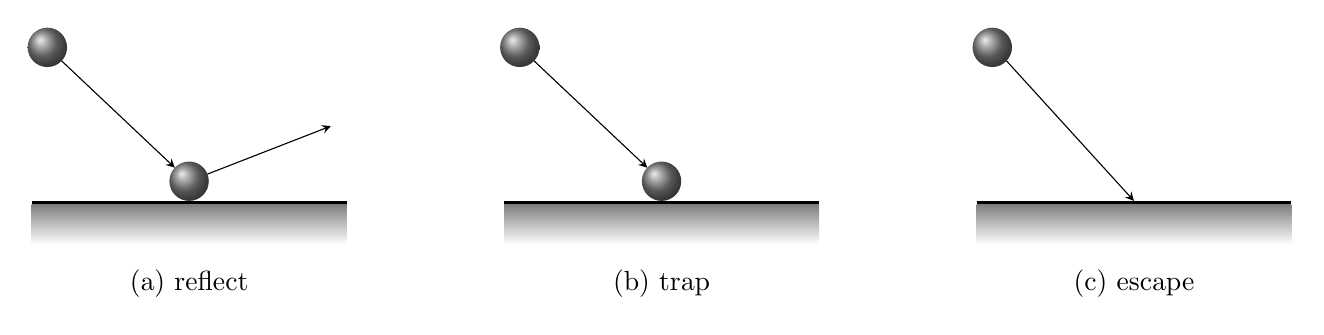
\begin{tikzpicture}
  [
    >=stealth,
  ]
  \draw [line width=0.1cm] (0,0) -- (4,0);
  \shade [shading=axis,shading angle=0] (0,0) rectangle (4,-0.5);
  \path [name path=in line]  (0.2,2) -- (2,0.3);
  \path [name path=out line] (2,0.3) -- (3.8,1);
  \path [name path=in circle] [shade,ball color=gray] (0.2,2) circle [radius=0.25];
  \path [name path=out circle] [shade,ball color=gray] (2,0.3) circle [radius=0.25];
  \draw [->][name intersections={of=in line and in circle, by=p1}, name intersections={of=in line and out circle, by=p2}] (p1) -- (p2);
  \draw [->][name intersections={of=out circle and out line,by=p3}] (p3) -- (3.8,1);
  \draw (2,-1) node {(a) reflect};
  
  \begin{scope}
  [xshift=6cm]
   \draw [line width=0.1cm] (0,0) -- (4,0);
    \shade [shading=axis,shading angle=0] (0,0) rectangle (4,-0.5);
    \path [name path=in line]  (0.2,2) -- (2,0.3);
    \path [name path=out line] (2,0.3) -- (3.8,1);
    \path [name path=in circle][shade,ball color=gray] (0.2,2) circle [radius=0.25];
    \path [name path=out circle][shade,ball color=gray] (2,0.3) circle [radius=0.25];
    \draw [->][name intersections={of=in line and in circle, by=p1}, name intersections={of=in line and out circle, by=p2}] (p1) -- (p2);
      \draw (2,-1) node {(b) trap};
    \end{scope}
    
      \begin{scope}
      [xshift=12cm]
       \draw [line width=0.1cm] (0,0) -- (4,0);
        \shade [shading=axis,shading angle=0] (0,0) rectangle (4,-0.5);
        \path [name path=in line]  (0.2,2) -- (2,0.3);
        \path [name path=out line] (2,0.3) -- (3.8,1);
        \path [name path=in circle] [shade,ball color=gray] (0.2,2) circle [radius=0.25];
        \path [name path=out circle] (2,0.3) circle [radius=0.25];
        \draw [->][name intersections={of=in line and in circle, by=p1}, name intersections={of=in line and out circle, by=p2}] (p1) -- (2,0.05);
          \draw (2,-1) node {(c) escape};
        \end{scope}
  
\end{tikzpicture}
\end{document}